\section{Introduction}
The idea of the brain as a network of interconnected neuronal elements has existed since the late 19th century. These neuronal elements (e.g. long-range fibers, synapses, subcellular processes) are anatomically organized in multiple scales of space to allow communications over multiple scales of time enabling perception, cognition and action \cite{Shepherd1991-ri,Rieke1997-ok,Russell2016-gt}. Recent advances in neuroimaging \cite{Chung2013-zb,Hagmann2005,Biswal2010-hk} along with large-scale projects opened new frameworks for studying the brain by modeling  brain connectivity as networks, or connectomes \cite{hcp1,zuo2014open,alexander2017open}. One of the main challenges in connectomics is to understand the network structures that link individual histories, such as the genome, developmental stage, or experience, to cognitive phenotypes, such as personality traits, behaviors, or disorders, which has been dubbed ``connectal coding''~\cite{vogelstein2019connectal}.

A connectome is defined as an abstract mathematical model of brain structure as a network, composed of two sets: vertices (or nodes) that represents a biophysical entity of the brain, and edges that represent connections, or communication, between pairs of vertices \cite{sporns2005human,Hagmann2005,vogelstein2019connectal}. Connectomes can have additional structures. For example, edges can have weights that describe the strength of connection, and have other attributes, such as physical location of the edge. Similarly, nodes can also have attributes, such as anatomical labels, shape and size. This capacity of connectomes as a brain model comes with challenges in their analysis. 

The first challenge is the choice of the representation of a connectome. Figure \ref{fig:intro_fig}a and \ref{fig:intro_fig}b shows two valid, but different representations of a human connectome. In Figure \ref{fig:intro_fig}a, the connectome is shown as a collection of vertices and edges in the classical graph theory perspective.
The vertices are organized by their location in the human brain, but this is only one choice of layout. There are infinitely many layouts that are equally valid, and, potentially, useful.
In Figure \ref{fig:intro_fig}b, the connectome is shown as a collection of numbers laid out in rows and columns as an ``adjacency matrix'' in the computer science perspective. In this view, a row/column pair is a vertex, and edges between vertices $u$ and $v$ are depicted by a non-zero entry in the corresponding element of the matrix. Consequently, the row identities are linked to column identities. Permuting both rows and columns together results in a ``different'' matrix, but they represent the same connectome. Nonetheless, the adjacency matrix is a useful representation of connectomes.

The second challenge is that connectomics data are different from typical Euclidean data in many ways. Some operations, such as addition and multiplication, are not well defined. What would it mean to add two connectomes together? Distance metrics are also not well defined, making comparisons between connectomes difficult. In the view of adjacency matrices, each entry is potentially related and dependent on other entries.

The third challenge is that connectomics data can be highly variable. For a graph with $n$ vertices, there are $n \choose 2$ possible edges so the number of unique graphs is $2^{n \choose 2}$. Figure \ref{fig:intro_fig}c shows the exponential growth in the number of unique graphs as the number of vertices increase. The large number of possible graphs makes characterizing and describing the graphs is difficult without statistical analysis of connectomics data.
% TODONE a third challege, there are many, eg, 2^n^2 of them with n vertices.  maybe worth showing that sequence in fig 1? maybe also for unlabeled? that there are so many means that we will really need statistics. 

Current connectomics analysis frameworks can be organized into four categories, each of which address the above challenges to various extents.
The first approach, and by far the most popular, is dubbed the bag of features. In this approach, a set of graph-wise or vertex-wise statistics that capture the structural aspects of networks are computed and compared \cite{Bullmore2010-ew,mhembere2013computing}. One major drawback to this method is that features are not independent of one another, making results from subsequent inference using these features difficult to interpret.
In the second approach, the bag of edges, each edge is studied individually. As a consequence, edges are treated independently, ignoring the other potential interactions \cite{Craddock2013-qs,Varoquaux2010-tc}. 
In the third approach, the bag of vertices, the vertices are studied while leveraging some structural information of the connectomes.
In the fourth approach, the bag of communities, the vertices are first organized into (typically) disjoint groups to form communities, and then edges within and across communities are studied. The last approach, the bag of networks, studies the connectomes as a whole to test for differences across groups or to classify connectomes.

While each of the frameworks provide complementary and meaningful insights into the connectomes, the underlying methodologies, and, thus, the interpretation of results can vary significantly. Statistical modeling of connectomes bridges the gap by providing a unified framework for studying connectomes. Conceptually, statistical models capture important differences within or among networks while considering the built-in structures and heterogeneity in networks \cite{Zheng2009-df,athreya2017statistical,arroyo2019inference, zhang2018network}. These differences are summarized by model parameters that can be used in a variety of subsequent inference tasks. 

This article is intended as a quantitative review of current connectomics analysis methods, and how statistical models can be incorporated to improve current analysis methods. We perform empirical investigations to demonstrate to what extent conclusions can be trusted as a function of the analysis method and the hypothesis in consideration. We vary parameters for the data, such as the generative model, sample size, and effect size, and hypothesis testing frameworks. Ultimately, the statistical modeling of networks uniquely provides a framework for meaningful and accurate testing and estimation for connectomics.

\begin{figure}
    \centering
    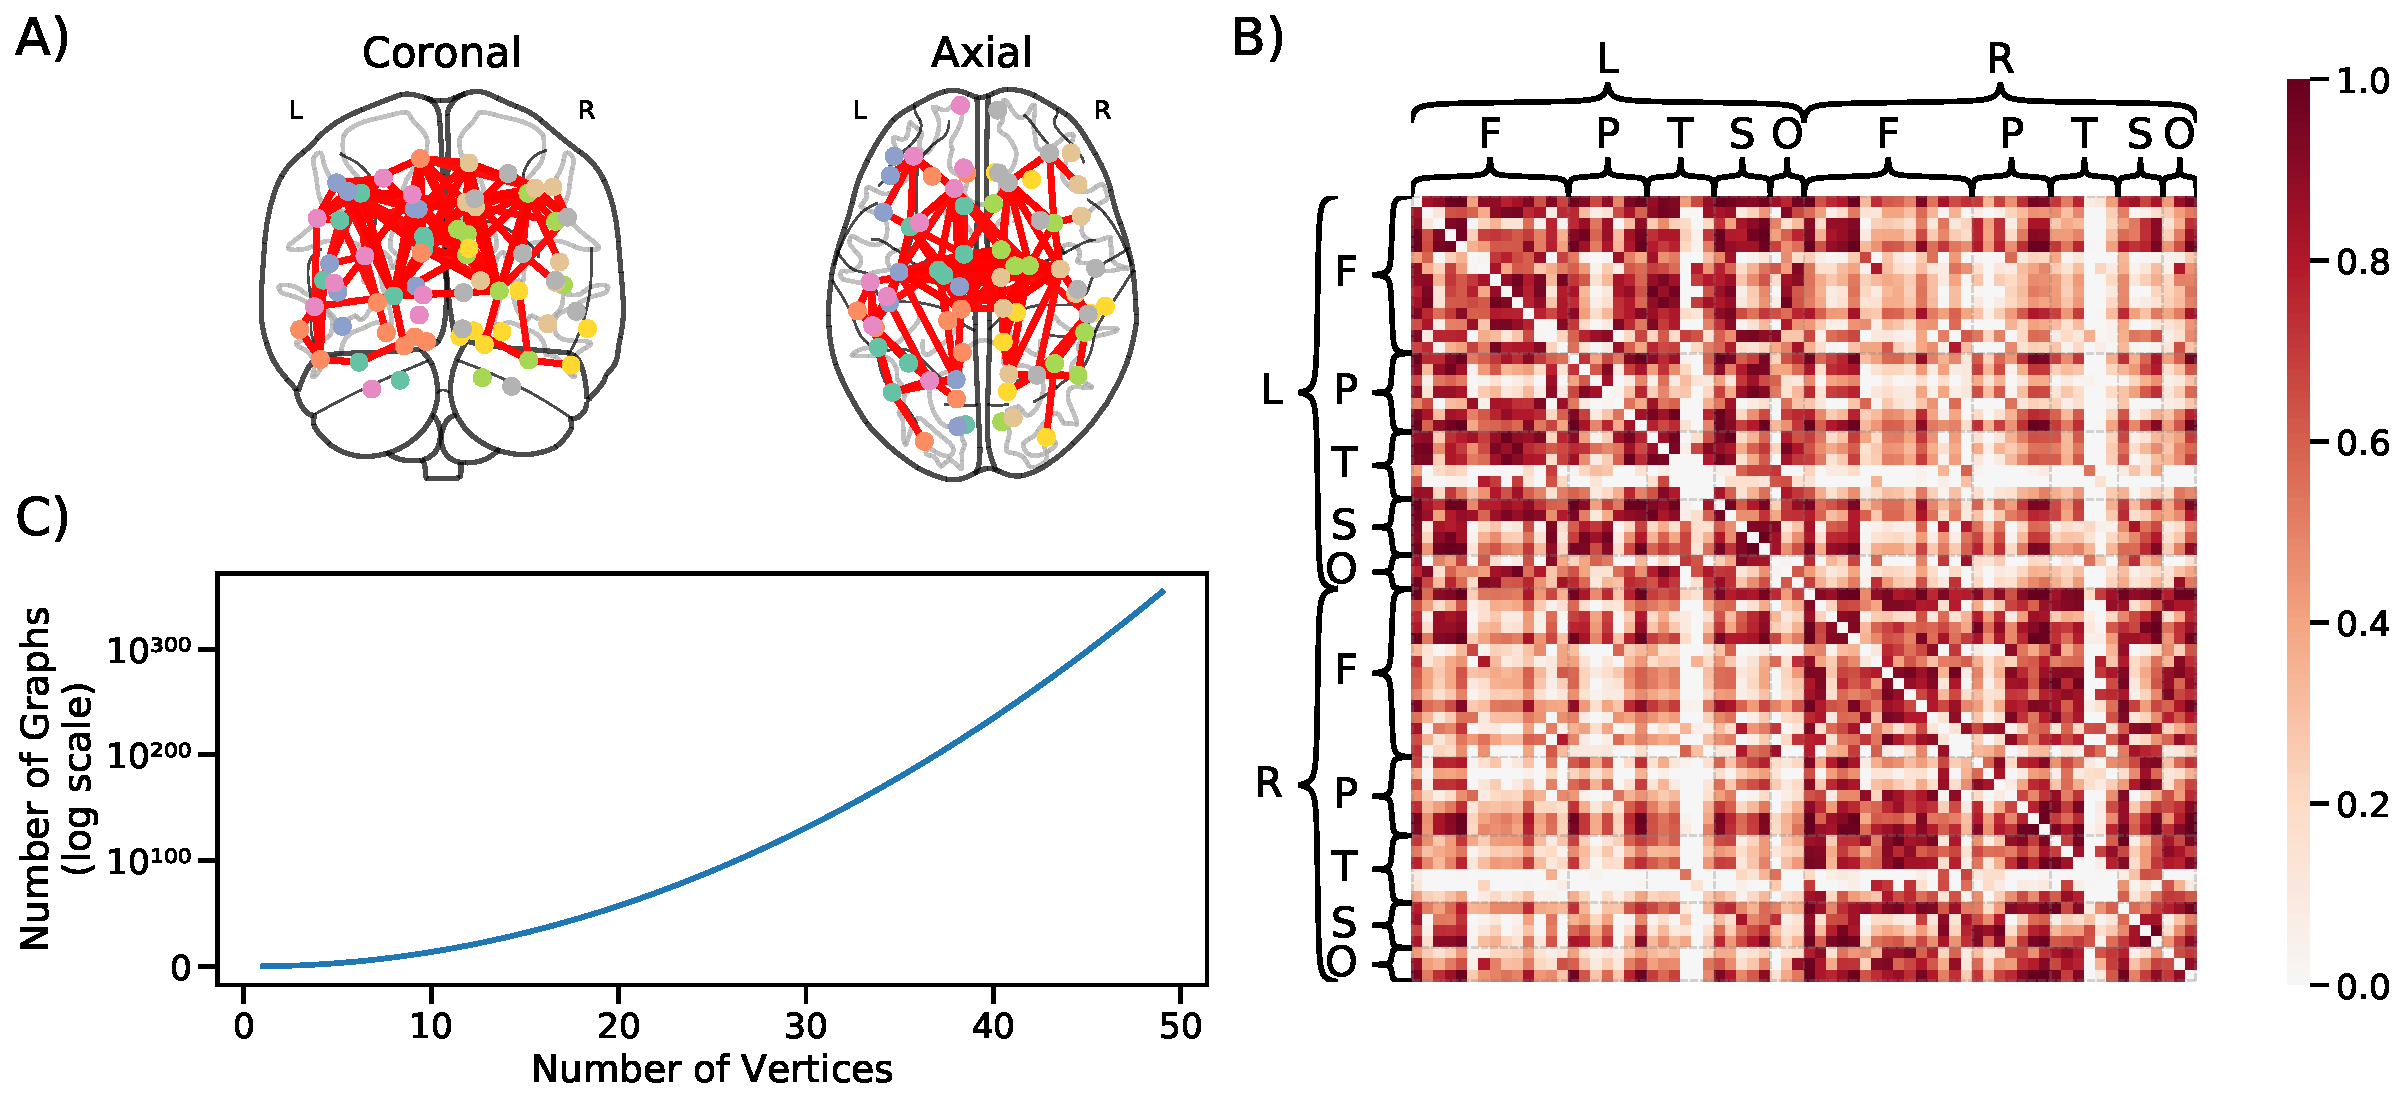
\includegraphics[width=\textwidth]{figures/dnd/intro}
    \caption{
    \textbf{Different Representations of a Connectome.} 
    Human structural connectome estimated from averaging 1059 human connectomes from the Human Connectome Project \cite{hcp1}.
    Vertices represent regions of the brain, and are assigned into right (R) and left (L) hemispheres and then further assigned into frontal (F), occipital (O), parietal (P), and temporal (T), and subcortical structures (S). 
    \textbf{a.} Connectivity shown in the coronal and axial views. Dots corresponds to the center-of-mass of the a region, lines correspond to connections, and line thickness corresponds to magnitude of the connection. Only the largest 5\% of edges are shown for visualization purposes. Note that infinitely many spatial arrangement of the vertices exist, and only one particular arrangement is being shown.
    \textbf{b.} Connectivity of the average structural connectome shown as an adjacency matrix, $\A$. The rows and columns are organized by hemisphere then further organized by sub-structures. However, given any permutation matrix $\Pbf$, the permuted adjacency matrix $\Pbf\A\Pbf^\top$ is still a valid matrix of original connectome. For a graph with $n$ vertices, there are $n^2$ permutations.
    \textbf{c.} The number of unique graphs grows exponentially as the number of vertices increases. The large number of graphs motivate statistical analysis to characterize and describe connectomes.
    } 
    \label{fig:intro_fig}
\end{figure} 